\chapter{Dicom-Presenter}
\vspace{-10mm}
My predecessor Bc. Pavel Neskudla began the development of an application for viewing images captured on Magnetic Resonance Imaging (MRI) unit in his Master's thesis\cite{neskudla}. It was a task given by the IKEM institute in Prague. IKEM institute specialists would utilize some application which was deployable on personal computers and which would display MRI images. It is possible to find such applications, but unfortunately these are mostly expensive commercial solutions or otherwise freeware applications and they do not reach quality requirements\footnote{See \cite[page~9]{flaska_bc} for an overview of available DICOM image viewers}. Within the framework of ongoing cooperation, IKEM asked the FNSPE faculty to develop such an application, which would meet their requirements. Moreover, in this case, the sponsor was allowed to raise unique functionality demands not accessible in other programs (See section \ref{requirements}).

\section{DICOM Standard}

DICOM is an abbreviation of Digital Imaging and Communications in Medicine, it is a standard for handling, storing and transmitting medical information\footnote{DICOM standard was created by  U.S. National Electrical Manufacturers Association\citesec{nema}.}. Namely, DICOM standard describes a file format for storing medical data and besides it describes a protocol for exchanging this data. DICOM standard uses common IT standards such as JPEG, TCP/IP, etc. \cite{dicombook}

The main reason DICOM was created was to avoid medical data confusion. DICOM files are equipped with a header including patient's information. This permanent attachment of header data to DICOM files should avoid random data substitution. There is information about the patient and the medical facility, as well as a diagnosis in the file header.

\subsection{DICOM Viewers}
\label{viewers}
DICOM software is very consumer-specific. Therefore, there are just a few DICOM image viewers available. According to \citesec{idoimaging} these are the most used DICOM viewers:

\begin{itemize}
  \setlength{\itemsep}{0pt}
  \setlength{\parskip}{0pt}
  \setlength{\parsep}{0pt}
\item \emph{Myrian}, Intrasense, \url{http://www.intrasense.fr/}
\item \emph{NovaPACS}, Novarad, \url{http://www.novapacs.com/}
\item \emph{K-Pacs}, Dr. med. Andreas Knopke, \url{http://www.k-pacs.net/}
\item \emph{DICOM Works}, Philippe PUECH, Loïc BOUSSEL, \url{http://dicom.online.fr/}
\item \emph{OsiriX}, OsiriX Foundation, \url{http://www.osirix-viewer.com/}
\item \emph{Aeskulap}, Alexander Pipelka, \url{http://aeskulap.nongnu.org/}
\item \emph{kradview}, David Santo Orcero, \url{http://www.orcero.org/irbis/kradview/}
\item \emph{SureVistaVision\texttrademark DICOM Viewer}, MS Technology, \url{http://www.ms-technology.com/medical-solutions/sure-vista-vision.html}
\item \emph{UniPACS},  \url{http://www.idoimaging.com/}
\item \emph{syngo Imaging}, Siemens, \url{http://www.medical.siemens.com/}
\item \emph{VR-Render}, IRCAD, \url{http://www.ircad.fr/softwares/vr-render/Software.php}
\item \emph{MicroDicom}, Simeon Antonov Stoykov, \url{http://www.microdicom.com/}
\end{itemize}

Unfortunately, Myrian, NovaPACS, syngo Imaging and SureVistaVision\texttrademark are commercial applications. Therefore, they are not suitable for use in IKEM institute. OsiriX is very powerful DICOM viewer but it is available only for Max OS X. Thus the variety of DICOM viewers is very limited.

All the DICOM viewers mentioned above are very similar in appearance. A program GUI is divided into a viewing area and a control area. The application can display a DICOM image in the viewing area or it can display a multi-planar reconstruction of the image. The control area offers image enhancing operations with the image displayed in the viewing area.

\begin{table}[ht]
	\captionsetup{tablename=Figures}
	\caption{DICOM viewers.}
	\centering
	\begin{tabular}{cc}
			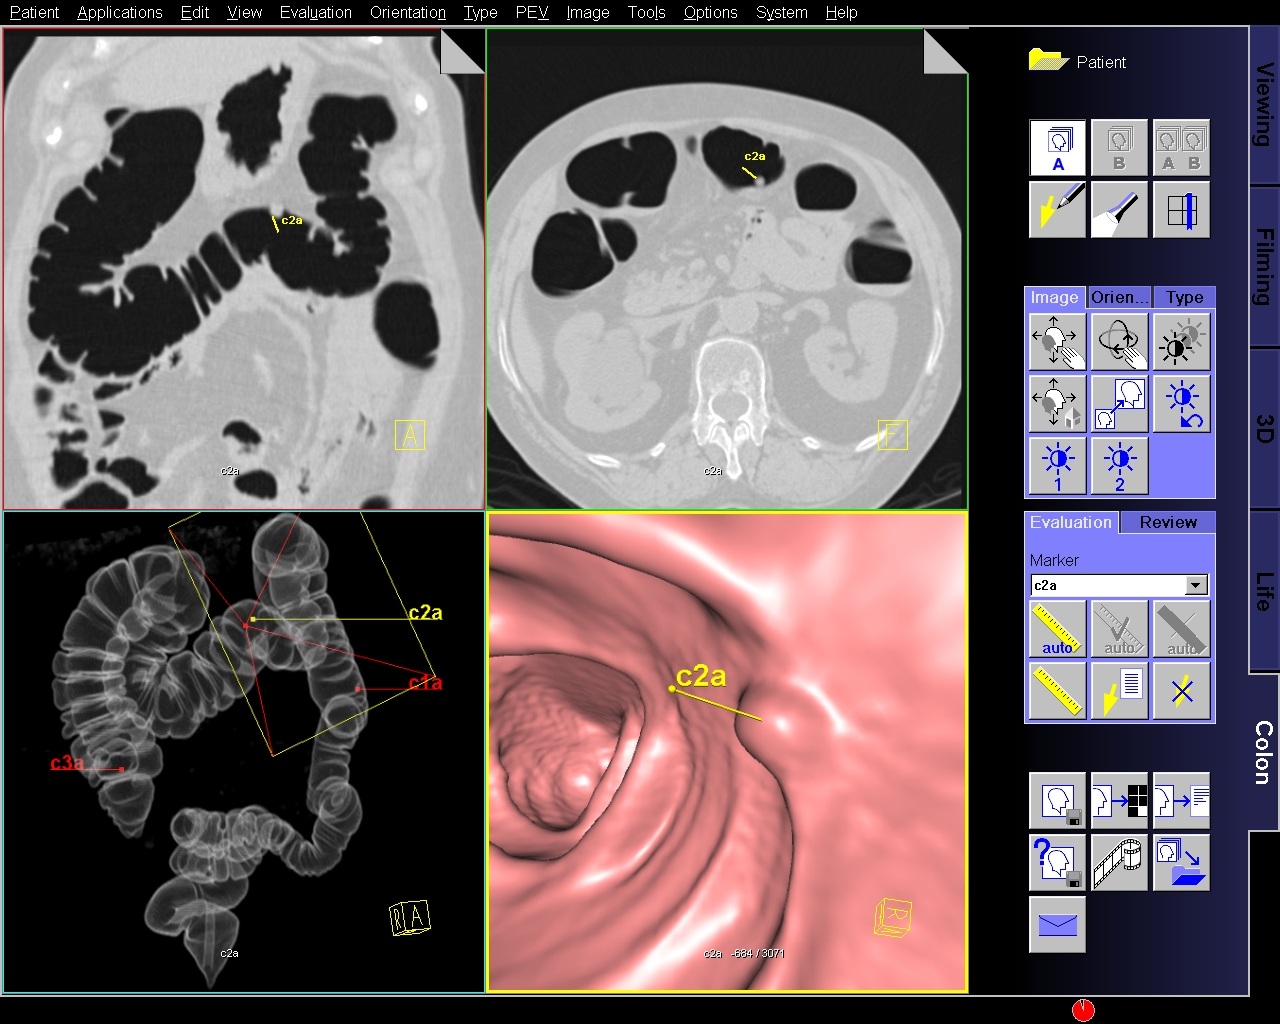
\includegraphics[width=0.5\textwidth,height=0.375\textwidth]{Text/IMG/01_Siemens.jpg}
		&
			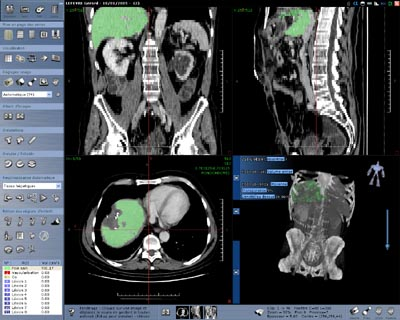
\includegraphics[width=0.5\textwidth,height=0.375\textwidth]{Text/IMG/01_Myrian.jpg}
		\\
			syngo Imaging~\citesec{siemens} & Myrian~\citesec{intrasense}	
		\\
			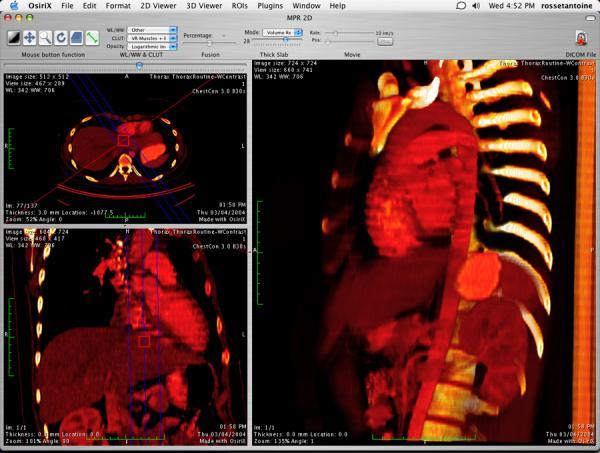
\includegraphics[width=0.5\textwidth,height=0.375\textwidth]{Text/IMG/01_OsiriX.jpg}
		&
			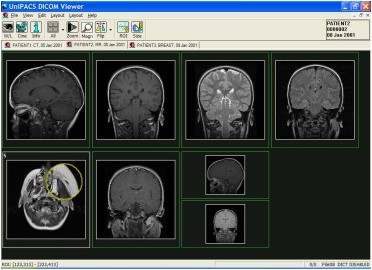
\includegraphics[width=0.5\textwidth,height=0.375\textwidth]{Text/IMG/01_UniPACS.jpg}
		\\
			OsiriX~\citesec{osirix} & UniPACS~\cite{idoimaging}
		\\
		\end{tabular}
\end{table}%




\section{Application Requirements}
\label{requirements}
The IKEM specialists requested a typical DICOM images viewer with a few more specific features not available in freeware programs. A typical DICOM viewer allows the user to open .dcm files and display it. In this case a .dcm file is a jpeg image equipped with a special header, where patient's information is included. MRI images are three-dimensional, thus user has to be able to select, which slice to be displayed. Some DICOM viewers offer a multi-planar image reconstruction. Other offered functions may vary.

There have been two specific requirements toward application functionality requested from IKEM specialists. These were not available in freeware DICOM applications. The most important function was the possibility to open several images at once and display them on the screen simultaneously. The user should be allowed to arrange images on screen to any possible layout he/she prefers. This functionality allows physicians to see two or more different MRI images on screen, so they can easily determine pathological changes of an observed organ. It is useful for studying, or for teaching.

There have also been requirements to record user's manipulation with images as a video. Then physician can prepare his presentation of images at home and play the video to their colleagues at a later point in time.

\section{Implementation}
After summarizing all the application requirements given by IKEM it was necessary choose appropriate technology for application implementation. The aim was to develop a GUI application capable of opening and displaying images, there are several ways to go, so it was the place for a discussion. 

The main question is which programming language to choose for the implementation. C\#, Java, C++ are the most popular programming languages for extensive GUI applications. C++ offers low level features and thus it offers very good performance. Java and C\# are both interpreted languages. Both were designed to be simple and robust. Although C\# and Java provide performance similar to C++ in overall tasks, still C++ attains better performance in tasks related to imaging\cite[Chapter~14]{csharpjavaperformance}. Therefore, C++ was chosen as a programming language for the Dicom-Presenter.

A Graphic User Interface of a C++ application is generally written with use of some library. It is possible to write a C++ GUI interface without an external library using only OS related function calls \footnote{A comparison of GUI interface written with and without external library can be found in Section \ref{noqt}}. There are more than ten widget toolkit libraries possible to be used for writing C++ GUI application. Qt\citesec{qthome} and GTK\citesec{qthome} are popular libraries used in many commercial applications and offering extensive possibilities for C++ application programming\cite[pages~413-416]{qtvsgtk}. Besides GUI creation Qt and GTK offers assistance with image manipulation, network access, xml parsing, etc. Both libraries are cross-platform. Finally, Qt was used because of better documentation offered by its author.

There was a research idea when creating Dicom-Presenter: check possibility of using GPU in this kind of application. Dicom-Presenter will have to handle with quite large graphic data\footnote{If an MRI image will consist of $50$ slices consisting of $512 \cdot 512$ pixels each, and each pixel will be saved within 2 bytes, then the three-dimensional image will be 26MB large\cite[page~121]{mrioverall}.} If GPU and its memory are able to handle this data, a significant performance enhancement could be reached. Therefore, OpenGL library was used for all image manipulation in Dicom-Presenter. It solves image storing, image manipulations and image rendering. Unfortunately, OpenGL brings occasional incompatibility with some hardware, which was unacceptable so the main goal of this project is to remove OpenGL from Dicom-Presenter. If OpenGL library would be replaced, then also dependencies on Cg toolkit library and plib library would also be removed. This would greatly simplify project compilation and lead to enhanced compatibility.



\section{Functionality}
\label{dicom-presenter}
Dicom-Presenter design is based on appearance of other DICOM image viewers. The goal was to display images and perform basic image manipulation. The application window can be divided into two main parts: a rendering part and a control part. The rendering part itself is divided into three sub-parts. Most of the space is naturally reserved for image rendering (later called Workspace). Bottom part is used for switching workspaces (later called Workspace Explorer). A side part or rendering window is used for accessing images stored in application memory (later called Image Explorer). Next to the rendering part is a control window which allows user to watch image  properties and adjust them numerically (later called Control Panel). 

The above described concept is very similar in appearance to other viewers unlike the part allowing workspace switching. It is a feature required by IKEM, that is not supported in any of DICOM viewers mentioned in Section \ref{viewers}.

The basic scenario of Dicom-Presenter work session can be described in the following way: After running the application user clicks ``Open Dicom Image'' button located on the control panel. Then the image preview appears in the Image Explorer (see Figures \ref{dicompresentergui}). By clicking the image preview, the image becomes a Selected Object. There is only one Selected Object in Dicom-Presenter at any one time. A key property of the Selected Object is that the Control Panel contains its information. Therefore, after declaring the opened image as selected a button called ``Create Image Copy'' appears in the Control Panel. By clicking the mentioned button, the image appears on the Workspace. To open next image, user clicks the appropriate button again. Afterwards, a second image preview appears in Image Explorer. Then the necessity of Image Explorer becomes apparent.

The user is allowed to freely customize the image arrangement on the Workspace. This is a notable feature in Dicom-Presenter. None of the DICOM viewers mentioned in Section \ref{viewers} offers it. Therefore, it was by request from IKEM that image layout has to be fully customizable. Images can be easily moved  by clicking any image at a proper place and dragging it on the Workspace.  It is a powerful user-friendly feature.

As was said before, Dicom-Presenter is intended to allow presenting images to other physicians. To avoid a need of picture manipulation during a presentation, a possibility of having more workspaces opened was implemented. Each workspace can be prepared before presenting and stored in the application memory.
 
\begin{table}[ht]
	\captionsetup{tablename=Figures}
	\caption{A scheme of Dicom-Presenter's GUI.\label{dicompresentergui}}
	\centering
	\begin{tabular}{m{0.5\textwidth} m{0.5\textwidth}}
			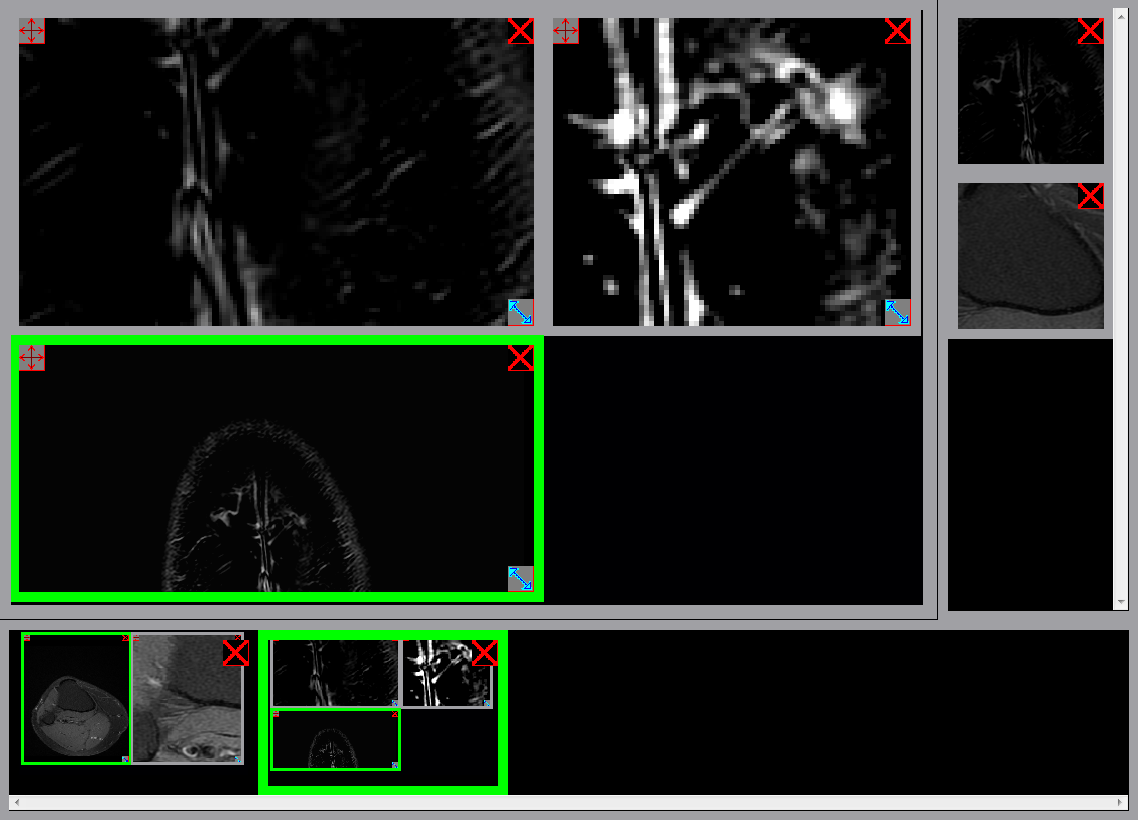
\includegraphics[width=0.5\textwidth]{Text/IMG/GUI_Screenshot.png}
		&
			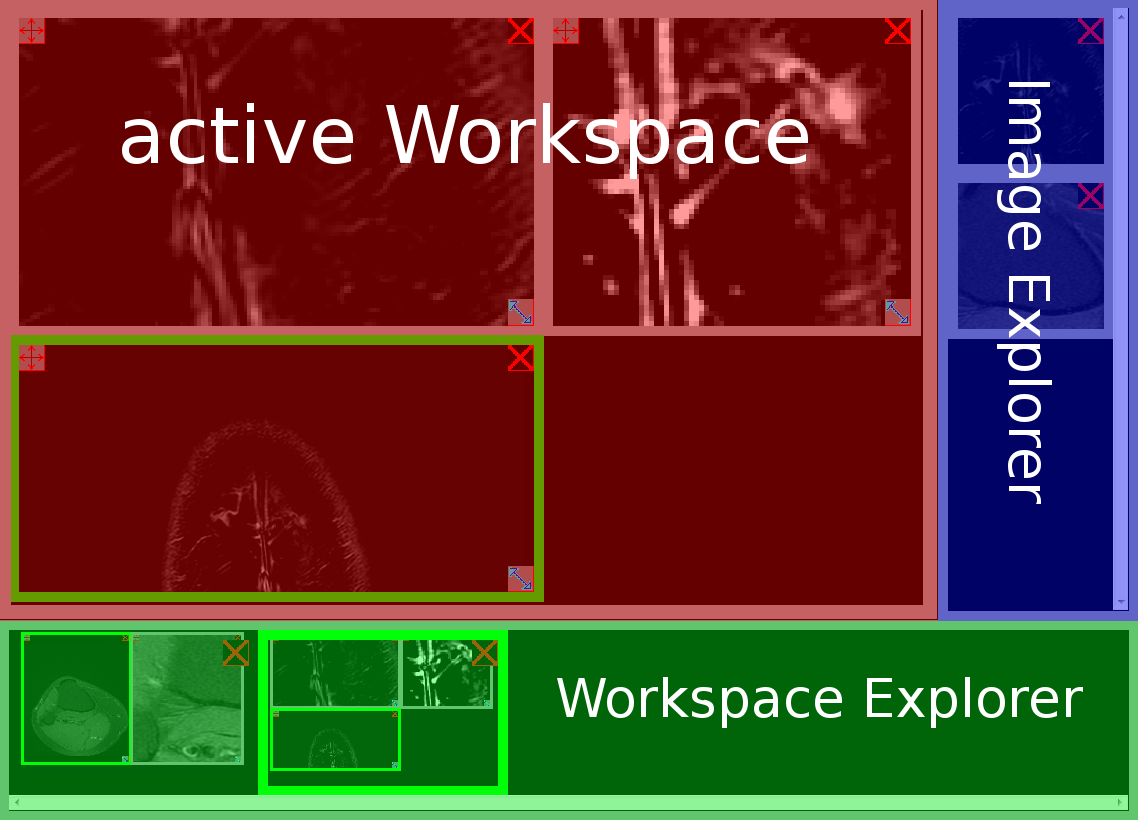
\includegraphics[width=0.5\textwidth]{Text/IMG/GUI_Screenshot1_English_Label1.png}
		\\
			A visual output of the application. & Three main objects present in the output window.
		\\
		\end{tabular}
\end{table}%